\documentclass[a4paper,14pt]{extreport}
\usepackage[utf8]{inputenc}
\usepackage[T1]{fontenc}
%\usepackage{lmodern}
\usepackage[english, russian]{babel}
\usepackage{indentfirst}
\usepackage{amssymb,amsfonts,amsmath,mathtext,cite,enumerate,float}
\usepackage[dvips]{graphicx}
\usepackage{titlesec}

\usepackage{geometry}
\usepackage{enumitem}
\geometry{left=2cm}
\geometry{right=2cm}
\geometry{top=0.5cm}
\geometry{bottom=2cm}

\titleformat{\chapter}[block]{\normalfont\bfseries}{\thechapter}{20pt}{}{}
%\addto\captionsrussian{\renewcommand{\chaptername}{}}
%\renewcommand{\thechapter}{}

\graphicspath{{images/}}

% Title Page
\title{Введение в дипломную работу}
\author{Елисеев Владислав}

\makeatletter
\bibliographystyle{unsrt}
\renewcommand{\@biblabel}[1]{#1.} 
\makeatother
\parindent=1.5cm

\sloppy
\hyphenation{STan-ford}

\newenvironment{compactlist}{
    \begin{list}
    {{$\bullet$}}
    {
        \setlength\partopsep{0pt}
        \setlength\parskip{0pt}
        \setlength\parsep{0pt}
        \setlength\topsep{0pt}
        \setlength\itemsep{0pt}                        
    }
}{
    \end{list}
}

\begin{document}
\begin{titlepage}

\begin{center}


\includegraphics[width=0.3\linewidth]{msu_title}

{\small
МОСКОВСКИЙ ГОСУДАРСТВЕННЫЙ УНИВЕРСИТЕТ имени М.В.~ЛОМОНОСОВА \\
ФАКУЛЬТЕТ ВЫЧИСЛИТЕЛЬНОЙ МАТЕМАТИКИ И КИБЕРНЕТИКИ \\
КАФЕДРА СИСТЕМНОГО ПРОГРАММИРОВАНИЯ
}
\end{center}

\vfill
\vfill
\begin{center}
\Large{\textbf{Введение в дипломную работу}} \\
~\\
\Large{Генерация моделей на унифицированном языке моделирования по описаниям предметных областей и~задач планирования}
\end{center}
\vfill
\vfill
\vfill
\vfill
\begin{flushright}
Исполнитель: \\
студент 527 группы Елисеев Владислав
\end{flushright}
\vfill
\begin{flushright}
Научный руководитель: \\
к.ф.-м.н. Малышко Виктор Васильевич
\end{flushright}
  
\vfill
\vfill
\vfill
\vfill
\begin{center}
  Москва\\
  2013
\end{center}  
\end{titlepage}

\newgeometry{top=2cm, bottom=2cm, left=2cm, right=2cm}

\setcounter{page}{1}
\linespread{1.25}
\normalsize

	Одна из задач в области искусственного интеллекта~--- задача планирования. Планированием называется процесс выработки последовательности действий, позволяющей достичь цели \cite{norwig-ai}. Задача планирования часто встает у агентов, которым нужно найти последовательность действий, выполнив которые он достигнет некоторой своей цели. Агентом можно назвать все, что воспринимает свою среду с помощью некоторых датчиков и воздействует на нее с помощью некоторых механизмов. Примерами использования планирования может служить следующее: планирование управлением механическими приводами робота-мусоросборника, планирование распределения транспортных средств для перевозок различных видов топлива и сырья на нефтеперерабатывающем заводе. 

	Контекст задачи планирования, модель мира, в котором возникает задача,  называется предметной областью.  
	
	В 1971 году для представления знаний о предметных областях был разработан формальный текстовый язык STRIPS \cite{strips}~--- STanford Research Institute Problem Solver. В этом языке выделяются три основных понятия~--- \textit{состояние среды} (мира), \textit{действие} (механизмы воздействия на среду), \textit{цель} (целевое состояние мира). Состояния задаются в виде некоторого набора фактов об объектах и отношениях между ними, которые считаются истинными в этом состоянии. Действия задаются с использованием набора ограничений на состояние (предусловие), и набора положительных и отрицательных фактов (эффекты). \textit{Предусловие} должно выполняться для того, чтобы применение действия было допустимым в данном состоянии. \textit{Эффект} задает то, как меняется состояние при применении действия~--- положительные факты добавляются к состоянию, отрицательные~--- удаляются. \textit{Цель}, или целевое состояние, задается как набор ограничений, которые должны быть удовлетворены в данном состоянии. Также в STRIPS вводится гипотеза замкнутости мира (CWA, \textit{Closed World Assumption}), которая означает, что факты, не перечисленные в описании состояния, считаются ложными.
	
	В 1987 году был предложен язык ADL~--- Action Description Language \textit{(язык описания действий)}~--- похожий на STRIPS, но включающий в себя еще несколько особенностей, из которых можно отметить следующие:
	\begin{itemize}
	    \item предположение об открытом мире - факты, не перечисленные в состоянии, считаются неизвестными;
	    \item возможность использования кванторов и дизъюнктов для задания цели;
	    \item возможность использования условных эффектов;
	    \item наличие встроенного предиката равенства для сравнения объектов;
	    \item возможность типизации переменных;
	    \item и т.д.
	\end{itemize}
    
    Помимо	языков STRIPS и ADL, вдохновленные ими, развивались и другие текстовые языки представления знаний, каждый из которых использовал свой синтаксис, семантику и другие возможности. В 1988 году появился язык PDDL\cite{pddl3}~--- Planning Domain Definition Language \textit{(язык описания предметных областей и задач планирования)}~--- как попытка стандартизации существующих на тот момент языков описания предметных областей и задач планирования. Также это сделало возможным создание IPC~--- International Planing Competition~--- международных соревнований по созданию планировщиков.  
    
    Рассмотрим пример PDDL-описаний для проблемы обедающих философов. За круглым столом сидят несколько философов, между каждой парой соседних из них лежит по одной вилке. В центре стола находится блюдо, которое хочет съесть каждый из философов, но может это сделать только если и в левой и в правой руке у него есть вилка. Философы могут выполнять следующие действия: они могут размышлять,  могут взять/положить вилку на стол в то место, откуда её взяли, могут приступить к еде. Задача состоит в том, чтобы спланировать действия философов так, чтобы никто из них не остался голодным, в случае, когда каждый подчиняется следующему алгоритму: после размышлений, философ становится голодным, затем он должен взять левую вилку (если она не занята), потом правую вилку (если она не занята), затем философ может перейти к еде. Пример описания предметной области на языке PDDL приведен далее:

\linespread{0.80}    
\begin{verbatim}
(define (domain dining_philosophers)
  ;; определяем предметную область
  
    (:requirements :typing :negative-preconditions)
      ;; указываем, какие возможности PDDL используются
      ;; типизация переменных
      ;; отрицания в предусловиях
    
    (:types
      ;; определяем типы
      Philosopher - object
      Fork - object
    )
    
    
    (:predicates
      ;; описываем типы отношений между объектами
      ;; в виде предикатов
      (right ?phi - Philosopher ?for - Fork) 
        ;; является ли вилка правой для философа
      (left ?phi - Philosopher ?for - Fork)
      (hold ?phi - Philosopher ?for - Fork)
        ;; держит ли философ вилку
      (hungry ?phi - Philosopher) ;; философ голоден
      (eat ?phi - Philosopher)    ;; философ ест
      (think ?phi - Philosopher)  ;; философ думает
      (hasLeft ?phi - Philosopher) ;; философ взял левую вилку
      (hasRight ?phi - Philosopher) ;; философ взял правую вилку
    )

    ;; затем идут описания действий    
    (:action getLeft
      ;; взять левую вилку относительно философа ?p1
      ;; вилка ?f находится между философами ?p1 и ?p2 
     :parameters (?p1 - Philosopher ?p2 - Philosopher ?f - Fork)
      ;; параметры операции
     :precondition 
       ;; предусловие
       (and
        (left ?p1 ?f)     ;; вилка слева от ?p1
        (right ?p2 ?f)    ;; справа от ?p2
        (hungry ?p1)      ;; философ голоден
        (not (hold ?p2 ?f));; другой философ не держит ту же вилку
       )
       
     :effect
       ;; эффект от применения операции
       (and
         (hasLeft ?p1)  ;; философ обладает левой вилкой
         (hold ?p1 ?f)  ;; философ взял конкретную вилку ?f
         (not (hungry ?p1)) ;; теперь философ не голоден
       )
    )
    
    ;; остальные действия описываются аналогично
    <..>
)

\end{verbatim}
\linespread{1.25}

    Описание задачи на языке PDDL состоит из перечисления объектов и их типов, указания начального состояния системы и набора ограничений на конечное состояние. Для задачи из предметной области обедающих философов пример приведен ниже:
  
\linespread{0.80}
\begin{verbatim}
(define (problem p1)
  ;; определяем задачу
  
  (:domain dining_philosophers)
      ;; указываем предметную область, для которой
      ;; сформулирована задача  
  
  (:objects
      ;; перечисляем объекты системы и их типы
      ;; три философа и три вилки      
      p1 - Philosopher
      p2 - Philosopher
      p3 - Philosopher
      f1 - Fork
      f2 - Fork
      f3 - Fork
  )
  (:init
      ;; задаем начальное состояние системы, 
      ;; т.е. значения предикатов на объектах системы
      ;; философы и  вилки расположены по часовой стрелке
      ;; первая вилка f1 находится слева от философа p1 и т.д.
      ;; все философы находятся в состоянии размышления
      (right p1 f3)
      (right p3 f2)
      (right p2 f1)
      (left p2 f2)
      (left p3 f3)
      (left p1 f1)
      (think p1)
      (think p2)
      (think p3)
  )
  (:goal
      ;; цель -- первый философ p1 приступил к еде.
      (eat p1)
  )
)
    
\end{verbatim}
\linespread{1.25}

    Графическое представление знаний может быть более удобным для использования людьми, нежели текстовое представлений. Для графического моделирования и удовлетворения нужд программной индустрии был разработан язык UML\cite{rambo-uml2}~--- Unified Modeling Language \textit{(унифицированный язык моделирования)}, но его возможности оказались шире, поэтому он используется и в других областях. Например, его можно использовать для представления знаний систем планирования в виде UML-моделей. Для задания дополнительных ограничений на UML-модели может быть использован язык OCL\cite{ocl}. Для создания UML-моделей существует множество редакторов, что делает возможность задания знаний среды и задачи планирования в графическом представлении более привлекательной. 
    
    В данной дипломной работе рассматривается следующая задача: по текстовым описаниям на языке PDDL требуется сгенерировать соответствующие им UML-модели. Получение UML-представления может быть полезно, так как:
    \begin{itemize}
        \item UML-модели более наглядны, составлять UML базы знаний могут эксперты, не знакомые с PDDL;
        \item UML-модель может быть отредактирована в UML-редакторе, и при необходимости её можно транслировать в другие языки (Java, PDDL, и~ др.);
        \item существуют средства валидации и исполнения UML-моделей для проверки корректности знаний\cite{use}; 
        \item существуют средства трансформации моделей, с помощью которых можно из UML-модели предметной области получить описания задач для этой предметной области.
    \end{itemize}


    Таким образом, предполагается создать программное средство, которое будет автоматизировать преобразование знаний систем планирования из текстового PDDL-представления в графическое представление в виде UML-моделей. Пусть $K$~--- знания системы планирования, $K = \langle D, T \rangle$, где $D$~--- знания о предметной области, $T = \{t_1, t_2, ...\}$~--- условия задач для данной предметной области. Знания о предметной области в свою очередь могут быть представлены в виде $D = \langle Types, Relations, Actions \rangle$, где $Types$~--- знания о типах объектов предметной области, $Relations$~--- знания о типах отношений между объектами, $Actions = {a_1, a_2, ...}$~--- знания о действиях $a_i$. Действие представляется в виде $a_i = \langle partypes, precond, effect \rangle$ и состоит из знаний о типах параметров, знаний о предусловии действия и эффекте от его применения. Типы параметров~--- упорядоченная последовательность типов $ partypes = \langle c_1, c_2, ..., c_n \rangle, c_i \in Types$. Действие $a$ применимо в том и только том состоянии $s$ для которого $precond_a(s,p) = True, s \in S, p \subset s$, где $S$~--- пространство всех состояний, $p = \langle o_1, o_2, ..., o_n \rangle$~--- фактические параметры действия с соответствующими типами. Эффект действия фактически задает новое состояние: $effect_a(s, p) = s' \in S$. Задачи представляются в виде $t_i = \langle Init, Goal \rangle$, где $Init \in S$~--- начальное состояние, $Goal: S \rightarrow \mathbb{B}$~--- ограничения на целевое состояние, отображение состояний в булево множество $\mathbb{B} = \{ True, False\}$. Любое состояние $s \in S$ представляется знаниями об объектах (экземплярах типа) и об отношениях между ними (экземпляры отношений), что иначе называется конфигурацией объектов и отношений, т.е. $s = \{o_1, o_2, ..., o_n, rel_1, rel_2, ..., rel_m\}$, $o_i$~--- экземпляр типа из $Types$, $rel_j$~--- экземпляр отношения из $Relations$.
    
    Знания в PDDL-представлении задаются следующим образом. $D_{PDDL} = \langle Types_{PDDL}, Relations_{PDDL}, Actions_{PDDL} \rangle$, где $Types_{PDDL}$~--- описания типов, $Relations_{PDDL}$~--- описания отношений в виде предикатов, $Actions_{PDDL}$~--- описания параметров действий, их предусловий и эффектов. Задачи  $t_{i, PDDL} = \langle Init_{PDDL}, Goal_{PDDL} \rangle$ описываются перечислением объектов с их типами, уточнением отношений между объектами.   Все это можно увидеть на примере, приведенном раннее.
    
    Знания в UML-представлении можно задать следующим образом в виде модели UML.  $D_{UML} = \langle Types_{UML}, Relations_{UML}, Attributes_{UML}, Actions_{UML} \rangle$, где $Types_{UML}$~--- UML-классы, соответствующие PDDL-типам, $Relations_{UML}$~--- UML-ассоциации между классами, соответствующие \textit{n-арным} ($n > 1$) между типами в PDDL, $Attributes_{UML}$~--- атрибуты классов, соответствующие \textit{унарным} предикатам PDDL, $Actions_{UML}$~--- описания параметров действий, их предусловий и эффектов. $Types_{UML}$ и $Relations_{UML}$ могут быть промоделированы с использованием диаграмм классов. $Actions_{UML}$ могут быть заданы, например, при помощи OCL. Задачи  $t_{i, UML} = \langle Init_{UML}, Goal_{PDDL} \rangle$ описываются с помощью объектов с указанием их типов, значений атрибутов и экземпляров ассоциаций. Задачи могут быть промоделированы с использованием диаграмм объектов. Состояние в UML может быть представлено как $ s \in S_{UML}, s = \{o_1, o_2, ..., o_n, rel_1, rel_2, ..., rel_m, atr_1, atr_2, ..., atr_l\}$, где $atr_i$~--- экземпляры атрибутов.
    
    В ходе работы создаваемого средства к представлению будет применяться ряд преобразований. Семантика знаний при этом должна сохраняться. Пусть $F$~--- описываемое преобразование, $F: K_{PDDL} \to K_{UML}$, $K_{PDDL}$~--- знания в исходном (текстовом PDDL-представлении), $K_{UML}$~--- база знаний в целевом представлении (в виде UML-модели). Преобразование $F$ можно представить в виде композиции преобразований $F = \langle F_T, F_R, F_A, F_C \rangle$, где $F_T: Types_{PDDL} \rightarrow Types_{UML}$~--- преобразование типов, $F_R: Relations_{PDDL} \rightarrow Relations_{UML} \cup Attributes_{UML}$~--- преобразование отношений, $F_A: Actions_{PDDL} \rightarrow Actions_{PDDL}$~--- преобразование действий, $F_C: t_{i, PDDL} \rightarrow t_{i, UML}$~--- преобразование задач. Преобразования должны обладать следующими свойствами:
    
    \begin{enumerate}
        \item В отображении типов (Рис.~\ref{img:property-types}) $F_T$ любому PDDL-типу должен соответствовать UML-класс, причем, разным типам должны соответствовать разные классы. Если типы связаны отношением тип-подтип, то в UML между ними должна быть связь обобщения:
    
        \begin{center}
            $\forall c \in Types_{PDDL} \Rightarrow F_T(c) \in Types_{UML}$; \\
            $\forall c_1, c_2 \in Types_{PDDL}, c_1 \neq c_2 \Rightarrow F(c_1) \neq F(c_2)$;
        \end{center}
                 

        
\begin{figure}[h]
    \hfill
    \begin{minipage}[h]{0.40\linewidth}
        {\raggedright
        \begin{verbatim}
    (:types
        thing - object
        stone - thing
    )
        \end{verbatim} 
        }
    \end{minipage}
    \hfill
    $\rightarrow$
    \hfill
    \begin{minipage}[h]{0.45\linewidth}
        \center{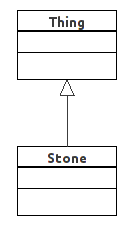
\includegraphics[width=0.5\linewidth]{property-types}}
    \end{minipage}
    \caption{Пример преобразования типов}
    \label{img:property-types}
\end{figure}
   

        \item В отображении отношений (Рис.~\ref{img:property-relations}) $F_R$ любому PDDL-предикату соответствует ассоциация UML либо атрибут UML-класса. Причем, если предикат \textit{унарный}, то он отображается в атрибут, иначе в ассоциацию; также разным предикатам соответствуют разные ассоциации/атрибуты:
    
        \begin{center}
        $\forall rel \in Relations_{PDDL} \Rightarrow F_R(rel) \in Relations_{UML} \cup Attributes_{UML}$;\\
        $\forall rel_1, rel_2 \in Relations_{PDDL}, rel_1 \neq rel_2 \Rightarrow F_R(rel_1) \neq F_R(rel_2)$; \\
        \end{center}

    
\begin{figure}[h]
    \hfill
    \begin{minipage}[h]{0.50\linewidth}
        {\raggedright
        \begin{verbatim}
    (:predicates
      (right ?phi - Philosopher 
          ?for - Fork)
      (hungry ?phi - Philosopher)
    )
        \end{verbatim} 
        }
    \end{minipage}
    \hfill
    $\rightarrow$
    \hfill
    \begin{minipage}[h]{0.45\linewidth}
        \center{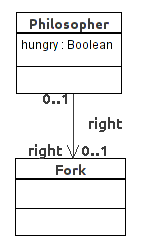
\includegraphics[width=0.5\linewidth]{property-relations}}
    \end{minipage}
    \caption{Пример преобразования отношений}
    \label{img:property-relations}
\end{figure}       


        \item 
        Введем вспомогательное отображение объектов в соответствующие типы $Type: o \in S \rightarrow Types$, отображение экземпляров отношений в соответствующие типы отношений $Relation: rel \in S \rightarrow Relations$, отображение экземпляров атрибутов в соответствующие атрибуты $Attribute_{UML}: atr \in S_{UML} \rightarrow Attributes_{UML}$, и отображение состояний $F_S: S_{PDDL} \rightarrow S_{UML}$,  для корректного определения которого потребуем выполнения следующих свойств:
       \begin{center}
        $\forall s = \{ o_1, ..., o_n, rel_1, ..., rel_m \} \in S_{PDDL} \Rightarrow$ \\ 
        $\Rightarrow F_S(s) = \{ o_1', ..., o_n', rel_1', ..., rel_k', atr_1, ..., atr_k \} \in S_{UML}$;  \\
                
        $\forall o_i \in s \Rightarrow F_T(Type_{PDDL}(o_i)) = Type_{UML}(o_i') $; \\  
        $\forall rel_i \in s \Rightarrow F_R(Relation_{PDDL}(rel_i)) = $
\[ = \left\{ 
    \begin{array}{l l}
        Attribute_{UML}(rel_k') & \quad \text{, $Relation_{PDDL}(rel_i)$~--- унарный предикат;} \\
        Relation_{UML}(atr_l) & \quad \text{, иначе;}
    \end{array}     
\right.\]
        \end{center}
        
        Тогда отображение задач (Рис.~\ref{img:property-tasks}) $F_C$ должно обладать следующим свойством корректности относительно отображения $F_S$ :
        
        \begin{center}
            $\forall t = \langle I, G \rangle \in T_{PDDL} \Rightarrow F_C(t) = \langle F_S(I), G' \rangle$; \\
            $\forall s \in S_{PDDL} \Rightarrow G(s) = True \Leftrightarrow G'(F_S(s)) = True $
        \end{center}
   
\begin{figure}[h]
    \center{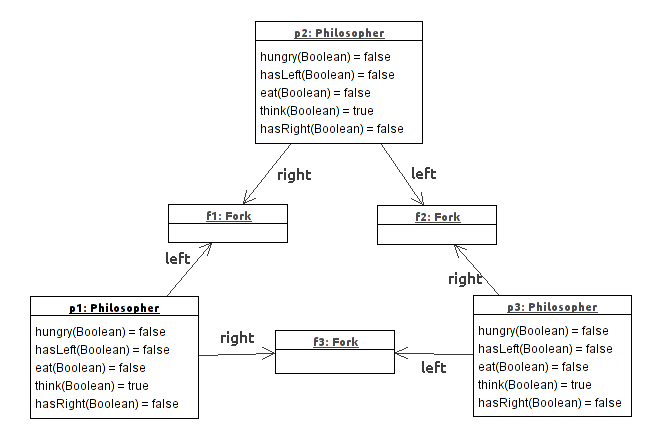
\includegraphics[width=1\linewidth]{property-tasks}}
    \caption{Пример преобразования задач}
    \label{img:property-tasks}
\end{figure}   
           
        \item
    Отображение действий (Рис.~\ref{img:property-actions}) $F_A$ должно удовлетворять следующим требованиям:
    \begin{center}
        $\forall a \in Actions_{PDDL} \Rightarrow F_A(a) \in Actions_{UML}$; \\    
    
        $\forall a_1, a_2 \in Actions_{PDDL}, a_1 \neq a_2 \Rightarrow F_A(a_1) \neq F_A(a_2)$; \\        
 
        $\forall a \in Actions_{PDDL}, partypes_a = \langle c_1, c_2, ..., c_n \rangle \Rightarrow F_A(a) = a', partypes_{a'} = \langle F_T(c_1), F_T(c_2), ..., F_T(c_n)\rangle$; \\
 
        $\forall a \in Actions_{PDDL}, \forall s \in S_{PDDL}, a' = F_A(a) \Rightarrow precond_a(s, p) = True, p \subset s \Leftrightarrow precond_{a'}(F_S(s), p') = True, p' = F_S(p)$, и \\
        
        $effect_{a'}(F_S(s), p') = F_S(effect_a(s, p)), p \subset s, p' = F_S(p) $;
    \end{center}            
       
\begin{figure}[h]
    \begin{minipage}[h]{1\linewidth}
        \center{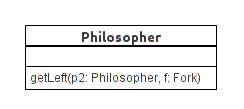
\includegraphics[width=0.5\linewidth]{property-actions}}    
    \end{minipage} \\
    \vfill
    {\centering $+$ \\ \medskip } 
        \begin{minipage}[h]{0.43\linewidth}
        
           \begin{verbatim}
    context Philosopher::getLeft(p2: Philosopher, f: Fork)
        pre 
            self.left = f 
            and p2.right = f 
            and self.hungry 
            and not p2.hold->includes(f)
        post
            self.hasLeft
            and self.hold->includes(f)
            and not self.hungry
           \end{verbatim}
        \end{minipage}

    \begin{center}
        \begin{minipage}{0.8\linewidth}
            \caption{Преобразование действий  на примере $getLeft$ с ограничениями на OCL}
        \end{minipage}    
    \end{center}

    \label{img:property-actions}
\end{figure}      

    \item
        Планом, решающим задачу $t = \langle I, G \rangle$ называется последовательность 
        \begin{center}
            $\langle s_1, a_1, p_1  \rangle, \langle s_2, a_2, p_2  \rangle, ..., \langle s_N, \emptyset, \emptyset \rangle \in Plans(t)$, \\ $s_i \in S, a_i \in Actions, p_i \subset s_i$
        \end{center}
        такая, что $s_1 = I, s_i = effect_{a_{i-1}}(s_{i-1}, p_{i-1}), i > 1$ и $G(s_N) = True$ где $Plans(t)$~--- множество планов, решающих задачу $t$.      
        
       
        Введем вспомогательное отображение планов $F_P: Plans_{PDDL}(t) \rightarrow Plans_{UML}(t)$:
            \begin{center}
                $\forall p = \langle s_1, a_1, p_1  \rangle, \langle s_2, a_2, p_2  \rangle, ..., \langle s_N, \emptyset, \emptyset  \rangle \in Plans_{PDDL}(t) \Rightarrow $\\
            $F_P(p) = \langle F_S(s_1), F_A(a_1), F_S(p_1)  \rangle, \langle F_S(s_2), F_A(a_2), F_S(p_2)  \rangle, ..., \langle F_S(s_N), \emptyset, \emptyset  \rangle \in Plans_{UML}(t) $  
            \end{center}
            
        Преобразование $F$ должно обладать свойством сохранения планов:
        
        \begin{center}
            $\forall t = \langle I, G\rangle \in T_{PDDL}, p \in Plans_{PDDL}(t) 
            \Leftrightarrow F_P(p) \in Plans_{UML}(t) $

        \end{center}
    \end{enumerate}
    
    Одной из сред поддержки процессов, связанных с планированием, является среда itSIMPLE\cite{itsimple}. В данной среде была решена обратная задача: трансляция UML моделей в PDDL описания. Для этого было предложено использовать специальную семантику некоторых UML-элементов. Так или иначе, средство не решает задачу, поставленную в данной работе.
    
    Подавляющее большинство инструментов, реализующих преобразование каких-либо текстовых данных в UML-модели, существует для работы с языками программирования, как правило, объектно-ориентированными, а не с языками представления знаний. Поэтому, использование этих инструментов для решения поставленной задачи невозможно. 
    
    Среди инструментов, работающих не только с языками программирования, можно выделить MoDisco. Данный инструмент позволяет создавать модели различных систем, используя специальные Discoverer'ы, которые на данный момент существуют в основном для Java-кода и JAR-архивов. Кроме того, данный проект находится в разработке и о создании PDDL-Discoverer'ов говорить не приходится. 
    
    Готовых средств, решающих данную задачу, нет, поэтому оправданно создание собственного средства. Вести разработку предполагается опираясь на универсальные фреймворки для создания средств компиляции и анализа. Для создания парсера PDDL грамматики возможно использование ANTLR~\cite{antlr}.
    

\newpage
\begin{thebibliography}{00}

\bibitem{norwig-ai}
\textbf{Рассел С., Норвиг П.} \textit{Искусственный интеллект: современный подход, 2-е изд.} М. : Вильямс, 2006. 1408 с.

\bibitem{strips}
\textbf{Fikes R., Nilsson N.} \textit{STRIPS: a new approach to the application of theorem
proving to problem solving // Artificial Intelligence}. 1971. 2. P. 189-208.

\bibitem{pddl3}
\textbf{Gerevini, A., Long, D.} \textit{Plan constraints and preferences in PDDL3.} Technical Report, Univ. Brescia, Italy, 2005. 12p.

\bibitem{rambo-uml2}
\textbf{Рамбо Дж., Блаха М.} \textit{UML 2.0. Объектно-ориентированное моделирование и разработка, 2-е изд.} СПб. : Питер, 2007


\bibitem{use}
\textbf{Gogolla M., Büttner F., Richters M.} \textit{USE: A UML-Based Specification Environment for Validating UML and OCL.} Science of Computer Programming, vol. 69, no. 1-3. 2007. pp. 27-34.


\bibitem{ocl}
\textbf{Warmer, Kleppe.} \textit{The Object Constraint Language: Getting Your Models Ready for MDA, Second Edition.} Addison-Wesley, 2003.

\bibitem{itsimple}
\textbf{Vaquero T. S., Tonaco R. et al.} \textit{itSIMPLE4.0: Enhancing the Modeling
Experience of Planning Problems.} Proceedings of the ICAPS 2012 System
Demonstration, São Paulo : s.n., 2012. pp. 11-14.

\bibitem{antlr}
\textbf{Terence Parr.} \textit{ The Definitive ANTLR 4 Reference}, 2013. 328p.

\end{thebibliography}

\end{document}          
